% !TEX encoding = UTF-8 Unicode
\begin{multicols}{3}[\section{Z-Wave}]

\rhead{Sebastian Lember}
\lfoot{20.05.2016}

\newrefsegment

\begin{tabular}{p{2,1 cm}p{2.7 cm}}
\textbf{Steckbrief}& \\
\end{tabular}
\rowcolors{1}{\topicolor!20}{}
\begin{tabular}{p{2,1 cm}p{2.7 cm}}
      Einsatz seit & 2014\\
      Frequenz"-bereich  & \SI{850}{\mega\hertz} - \SI{950}{\mega\hertz}\\
      Datenrate & \SI{100}{kB/s}, \SI{40}{kB/s}, \SI{9,6}{kB/s}\\
      Verbreitung & Weltweit, Z-Wave Allianz\\
      Reichweite & \SI{40}{\metre} (Gebäude), \SI{200}{\metre} (Freigelände)\\
      Modulation & FSK\\
      Sendeleistung & \SI{25}{\mega\watt}\\
\end{tabular}
\par
%Source http://www.fh-bingen.de/fileadmin/user_upload/Lehrende/Kilsch_Dieter/internet/projekte/TedoSchStiUnits.pdf -> Seite 9 findet ihr alle verwendbaren Einheiten, wie:
%\SI{Zahl}{\mega\hertz} oder \SI{Zahl}{\mili\metre}
%Ich weiß ehrlich gesagt nicht welche Einheiten ihr im Text genau braucht, aber in dem Dokument und mit obigen Beispiel sollte es umsetzbar ein.
\subsection*{Überblick}
\begin{wrapfigure}{r}{0.4\linewidth}
  \vspace{-20pt}
  \begin{center}
  	\hspace{-20pt}
    
\includegraphics[width=1\linewidth]{Kapitel/Z-Wave/Grafiken/logo.jpg}
  \end{center}
  \vspace{-15pt}
\end{wrapfigure}
Z-Wave ist ein weltweit verbreiteter, drahtloser Kommunikationsstandard für Heimautomation. Entwickelt wurde er von zwei dänischen Ingenieuren und der Firma Zen-Sys. 2005 wurde die Z-Wave Allianz gegründet und 2009 übernahm Sigma Designs die Firma Zen-Sys. Ziel ist es einen Kommunikationsstandard mit niedrigem Energieverbrauch und hoher Sicherheit bereitzustellen. Durch eine umfassende Spezifikation des Standards wird eine hohe Interoperabilität aller mit Z-Wave kommunizierenden Produkte gewährleistet.

\subsection*{Technische Erläuterung}
Der Z-Wave Protokoll beschreibt die Kommunikation einzelner mit Z-Wave ausgerüsteten Produkte.
Die Entwicklung dieser Produkte geschieht auf Basis eines SOC (Z-Wave-System-on-a-Chip-ASICs). Der SOC enthält einen Funk-Transceiver, einen Mikro-Controller, einige Peripherie-Schnittstellen und die Softwarebibliothek zur eigentlichen Kommunikation zwischen den Geräten. Die PHY- und MAC-Schichten des Z-Wave Protokolls sind seit 2012 werden durch den G.9959 Standard der ITU-T definiert. 

Z-Wave benutzt Funkfrequenzen zwischen \SI{850}{\mega\hertz} und \SI{950}{\mega\hertz}. Der Vorteil dieser Funkfrequenzen liegt darin, dass sie eine besser Durchdringung von Wänden liefern, als das weit verbreitete \SI{2,4}{\giga\hertz} Band. Allerdings gibt es keine einzelne weltweit verfügbare Funkfrequenz in diesem Frequenzbereich gibt. In Europa und Asien werden daher Frequenzen des SDR-Bandes (\SI{868,4}{\mega\hertz} bzw. \SI{869}{\mega\hertz}) genutzt. Die Alternativen Frequenzen in Amerika liegen im ISM-Band (Nordamerika: \SI{908}{\mega\hertz}, Südamerika: \SI{921}{\mega\hertz}. Außerdem nutzt Z-Wave eine FSK (Frequency Shift Keying), womit Datenraten von \SI{100}{kB/s}, \SI{40}{kB/s}, \SI{9,6}{kB/s} erreicht, die anhand der Funksituation dynamisch umgeschaltet werden.

Die Adressierung der Geräte innerhalb eines Netzes geschieht über den Primärcontroller. Dieser vergibt eine \SI{4}{Byte} lange Home ID und eine \SI{1}{Byte} lange Node ID, welche nur innerhalb des Netzes gültig ist. Damit können auch mehrere Netze parallel betrieben werden. Der Primärcontroller ist in kleinen Netzen meist eine Funkfernbedienung, in größeren Netzen verwendet man hingegen eine Zentralsteuerung mit IP-Zugang, der dann die Steuerung der Geräte übernimmt.

Die Kommunikation der einzelnen Geräte erfolgt über eine Zweiwege-Kommunikation, die eine Rückbestätigung erwartet. Kommt es zu einem Fehler, so wird der Sendevorgang bis zu 3 mal wiederholt. Z-Wave Geräte können Daten mit bis zu 4 Zwischen-Hops zu anderen Geräten im Netz weiterleiten. Dabei kann jedes Gerät, welches netzbetrieben ist als Router fungieren. Somit entsteht ein vermaschtes Netzwerk, dessen Routen über den Primärcontroller gesteuert wird.

\begin{Figure}
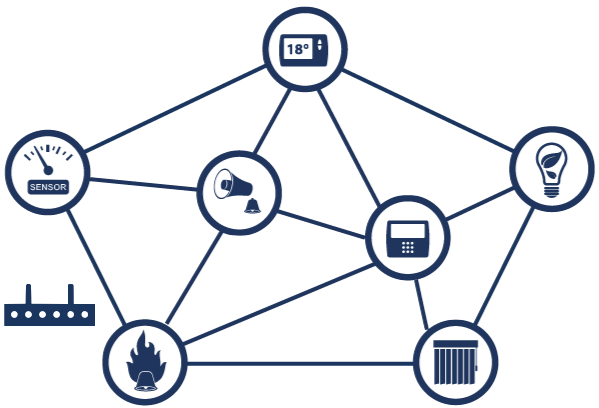
\includegraphics[width=\linewidth]{Kapitel/Z-Wave/Grafiken/z-wave_mesh.png}
\captionof{figure}{Vermaschung Z-Wave Netz~\cite{zwave.1}}
\label{fig:zwave_mesh}
\end{Figure}

\subsection*{Einsatz}
Z-Wave findet hauptsächlich in der Heimautomation gebrauch. Hierzu werden zertifizierte Geräte miteinander über den Funkstandard vernetzt und kommunizieren untereinander.

Mittels dieser Vernetzung kann man die Geräte manuell über eine App ansprechen und somit die gewünschte Aufgabe ausführen zu lassen, wie zum Beispiel das Licht anschalten oder den Rolladen hoch lassen. Zudem können die Geräte auch untereinander kommunizieren, um auf einen Sensor zu reagieren. Somit kann zum Beispiel über einen Lichtsensor automatisch der Rolladen runter- und hochgelassen werden oder mittels eines Temperatursensors die Heizung gesteuert werden.

Weitere Anwendungsmöglichkeiten sind:
\begin{itemize}
	\item Lichtsteuerung
	\item Klimatechnik
	\item Sicherheitssysteme
	\item Heimkinos
	\item Automatische Rolläden
	\item Steuerung von Pools
\end{itemize}

\subsection*{Anbieter und Gremien}
Urprünglich wurde Z-Wave von der dänischen Startupfirma Zen-Sys im Jahre 2001 entwickelt. Mittlerweile wird der Standard von der Z-Wave Allianz weiterentwickelt. Die Z-Wave Allianz ist ein Zusammenschluss von Herstellern und Dienstleistern, die die durch Z-Wave spezifizierten Produkte entwickelt und herstellt. Die Allianz hat Ihren Sitz in Milpitas/Kalifornien. Hauptmitglieder (sogenannte „Principal Members“) sind Fakro, Linear Technologies, Ingersoll-Rand, Jasco Products Company, Evolve und Sigma Designs. \cite{zwave.2} Die Z-Wave Allianz zertifiziert zudem die Produkte, die mit Z-Wave hergestellt werden, um die richtige Implementierung und die Interoperabilität der einzelnen Produkte zu gewährleisten.

\end{multicols}
\newpage

\section*{Historische Entwicklung}
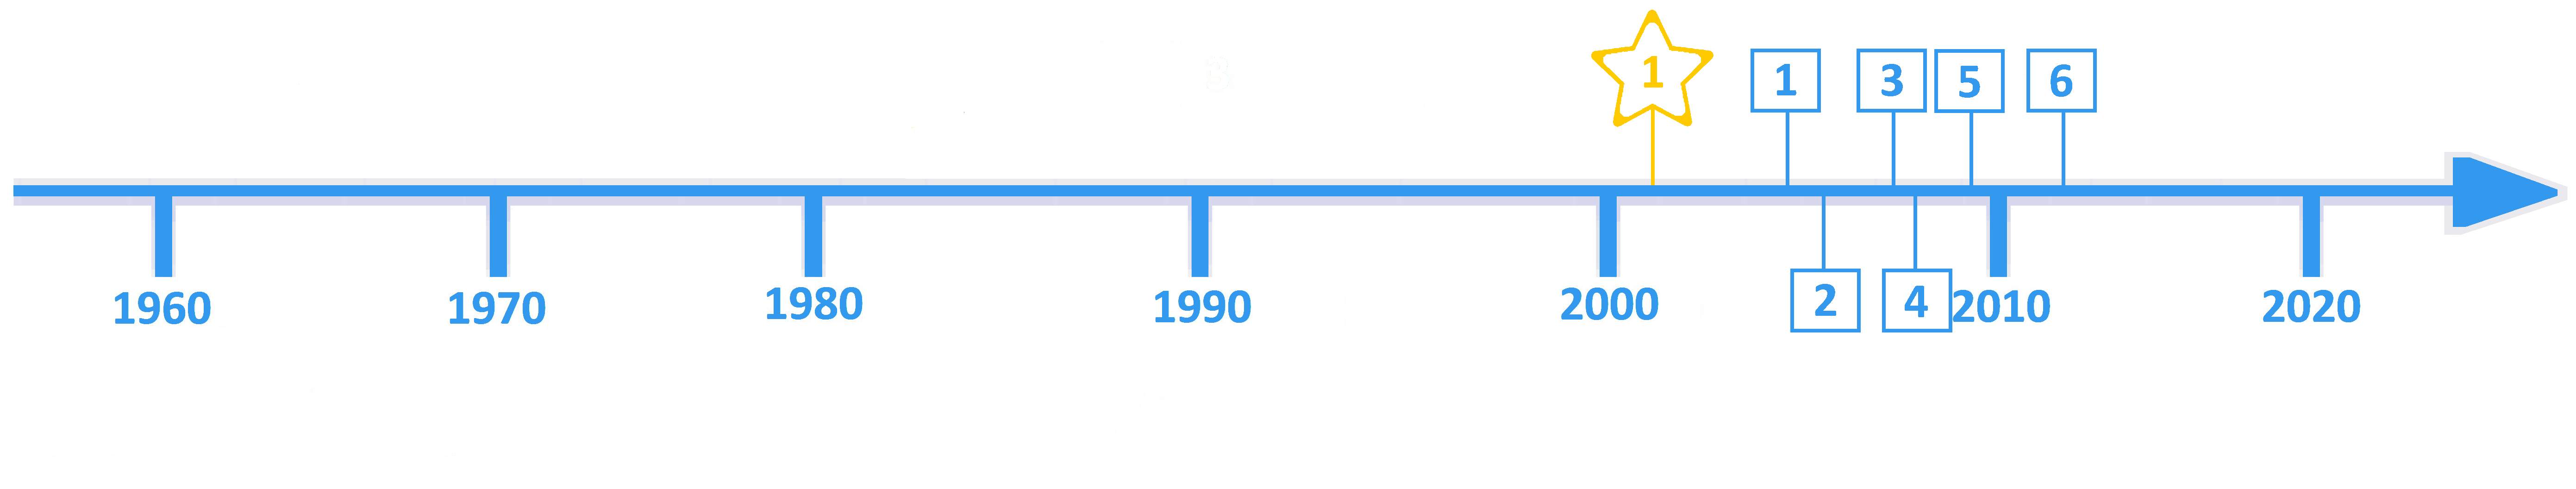
\includegraphics[width=\textwidth]{Kapitel/Z-Wave/Grafiken/Zeitstrahl.jpg}
\par
\noindent
\rowcolors{2}{}{\topicolor!20}
\begin{tabular}{p{0.5 cm}p{1.5 cm}p{15.55 cm}}
	Nr. & Datum & Entwicklungsschritte\\
	1 & 2001 & Entwicklung von Z-Wave durch zwei dänische Entwickler, die eine eigene Hausautomation auf den Markt bringen wollten.\\
	2 & 2004 & Die ersten Produkte kamen auf den Markt.\\
	3 & 2005 & Die Z-Wave Allianz wurde gegründet.\\
	4 & 2007  & Die ersten europäischen Z-Wave Produkte wurden vom dänischen Hersteller Danfoss produziert.\\
	5 & 2008 & Entwicklung der ersten deutschen Z-Wave Geräte von der Firma Merten GmbH.\\
	6 & 2009 & Übernahme durch Sigma Designs.\\
	7 & 2012 & Die Protokollschichten von Z-Wave sind im ITU-T Standard G.9959 definiert.\\
\end{tabular}
\par
\begin{multicols}{3}

Im Jahre 2001 wurde Z-Wave von einem dänischen Startup Unternehmen mit zwei Entwicklern entwickelt. Diese hatten zum Ziel eine eigene Heimautomationslösung auf den Markt zu bringen. Die Funktechnik wurde an andere Unternehmen verkauft, die dann die Geräte gebaut haben. Die ersten Produkte kamen im Jahr 2005 auf den Markt. In Europa war der erste Entwickler von Z-Wave Geräten im Jahr 2007 und in Deutschland im Jahr 2008. 

2005 wurde die Z-Wave Allianz gegründet. Diese spezifiziert den Standard und zertifiziert die Geräte um Interoperabilität zu gewährleisten. Die Firma Sigma Designs übernahm 2009 die Firma Zen-Sys.

\subsection*{Ausblick}
Da Heimautomation in Zukunft immer beliebter werden wird und auch immer mehr Privatkunden ihr zu Hause immer mehr automatisieren wollen, ist die Entwicklung solcher Standards wie Z-Wave sehr zukunftssicher. 

Z-Wave bietet einige Vorteile gegenüber anderer Funktspezifikationen, wie eine bessere Wanddurchdringung und weniger Verluste durch Reflexionen, hat allerdings auch Nachteile, wie eine geringere Datenrate und keine einheitliche Frequenz weltweit. Allerdings setzen immer mehr Unternehmen die Heimautomation produzieren auf den Z-Wave standard.
\printbibliography[segment=1,heading=subbibliography]
\end{multicols}

\newpage
